\section{Why Visible Events Can Have Ambiguous Sources}
\label{sec:narrative-information}

The continuous results raise a separate physical question: can these
measurements distinguish the candidate sources at all? A good state
estimate does not answer it. Different interventions can produce similar
histories after fitting their severity and initial state
\cite{eriksson2013diagnosability,scharf1994matched}.

For a response $s_h$ at a specified severity and context, its distance to
an admitted competitor is
\begin{equation}
 d_h^2=\min_{j\ne h}\ \min_{\eta_j\in\mathcal A_j}
      \|s_h-s_j(\eta_j)\|_{\Sigma^{-1}}^2.
 \label{eq:narrative-separation}
\end{equation}
The set $\mathcal A_j$ specifies allowed severity, sign and nuisance
coordinates. If zero severity is admitted, different support families can
meet at the no-event boundary. Unrestricted amplitude minimization would
then give a misleading source-separation interpretation. Under a common
Gaussian law, coincident means cannot be distinguished at that
intersection. Small distances indicate a noise-sensitive problem, not a
universal error formula or an online uncertainty certificate.

A separate archived load-only experiment illustrates observed ambiguity. It uses
32 rectangular voltage/current coordinates, known onset and known operating
context. Its original amplitude-integrated batch score compares 137
zero-, one- and two-source supports on \GlobalPhysicalTrajectories{} fresh
nonlinear trajectories. It is a different estimator and evidence contract
from the causal bank. Its scores require the normalization qualification
below before being interpreted under the originally declared priors.

\begin{figure*}[t]\centering
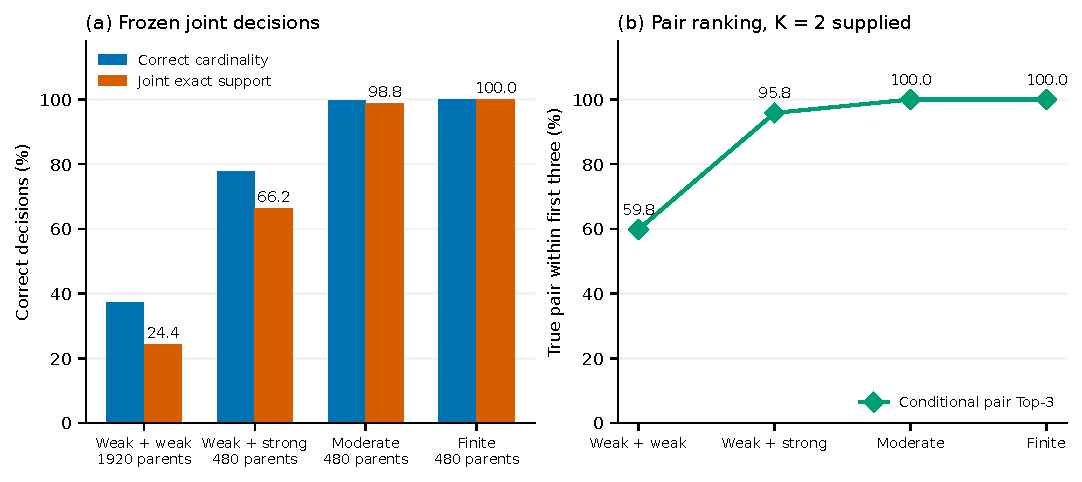
\includegraphics[width=.93\textwidth]{figures/generated/narrative_resolution.pdf}
\caption{Archived load-support outcomes, not causal R11 accuracy. Left: cardinality and joint exact-source decisions of the frozen 137-support implementation. Right: Top-3 rank restricted to the 120 pairs, conditional on knowing that two sources occurred; it is a different decision contract. Labels give independent physical trajectories, each replayed with three noise seeds. The evidence-normalization audit below qualifies the cardinality prior; these curves are not corrected-prior results or proof of an information-theoretic limit.}
\label{fig:narrative-resolution}\end{figure*}

Exact-support Top-1 increases from \GlobalWeakTopOne{} for weak pairs to
\GlobalFiniteTopOne{} for finite pairs (Fig.~\ref{fig:narrative-resolution}).
A visible intervention therefore need not yield a reliable location in
this implementation. Top-3 in the archive ranks only pair supports,
whereas Top-1 also requires the full bank to select two sources. They
must not be compared as though only the number of returned labels changed.
These observed errors do not separate insufficient information from model,
prior or numerical error; that separation requires an exact-response control.

The archived implementation also requires a prior qualification. Its
single-source integral carries an extra factor $1/(2\pi)$ relative to
the null and pair integrals, giving an effective cardinality prior
proportional to $(0.20,0.50/(2\pi),0.30)$ instead of the originally
declared $(0.20,0.50,0.30)$. A zero-response control on the historical
code exposed this difference. An isolated successor restores the declared
prior and passes independent linear-Gaussian checks for all 136 event
supports; its physical performance has not been recomputed. Figure~\ref{fig:narrative-resolution}
retains the archived implementation's outcomes. This issue does not alter
the local R11 amplitude integral, checked separately
by numerical quadrature.

Longer history and different PMUs may help discrimination, but these
curves do not certify an online uncertainty or abstention rule. Exact
replay of the auxiliary study requires restoring source arrays absent
from this artifact copy; no newly fitted dictionary replaces them.
Detailed state-reconstruction studies remain supporting evidence rather
than extra event-diagnosis scores.
